% Full instructions available at:
% https://github.com/elauksap/focus-beamertheme

\documentclass{beamer}
\usetheme[numbering=progressbar]{focus}
\usepackage{tikz}
\usetikzlibrary{positioning}
\usetikzlibrary{shapes,arrows}
\usepackage{transparent}
\usepackage{fancyvrb}
\usepackage{listings}
\definecolor{main}{RGB}{47, 161, 219}
%\definecolor{textcolor}{RGB}{128, 128, 128}
\definecolor{background}{RGB}{240, 247, 255}
\definecolor{textcolor}{RGB}{85, 87, 83}
\title{D4 Project}
\subtitle{Open and collaborative network monitoring}
\author{Alexandre Dulaunoy - Sami Mokaddem}
\titlegraphic{
\includegraphics[scale=0.20]{d4-logo.pdf}}
\institute{Team CIRCL \\ \url{https://www.d4-project.org/}}
\date{2019/03/29}

\begin{document}
    \begin{frame}
        \maketitle
    \end{frame}

\begin{frame}
        \frametitle{Problem statement}
        \begin{itemize}
                \item CSIRTs (or private organisations) build their {\bf own honeypot, honeynet or blackhole monitoring network}
                \item Designing, managing and operating such infrastructure is a tedious and resource intensive task
                \item {\bf Automatic sharing} between monitoring networks from different organisations is missing
                \item Sensors and processing are often seen as blackbox or difficult to audit

        \end{itemize}
\end{frame}


\begin{frame}
 \frametitle{Objective}
 \begin{itemize}
         \item Based on our experience with MISP\footnote{\url{https://github.com/MISP/MISP}} where sharing played an important role, we transpose
                 the model in D4 project
         \item Keeping the protocol and code base {\bf simple and minimal}
         \item Allowing every organisation to {\bf control and audit their own sensor network}
         \item Extending D4 or {\bf encapsulating legacy monitoring protocols} must be as simple as possible
         \item Ensuring that the sensor server has {\bf no control on the sensor} (unidirectional streaming)
         \item Don't force users to use dedicated sensors and allow {\bf flexibility of sensor support} (software, hardware, virtual)

 \end{itemize}
\end{frame}

\begin{frame}
        \frametitle{(short) History}
 \begin{itemize}
        \item D4 Project (co-funded under INEA CEF EU program) started - 1st November 2018
        \item D4 encapsulation protocol version 1 published  - 1st December 2018
        \item v0.1 release of the D4 core\footnote{\url{https://www.github.com/D4-project/d4-core}} including a server and simple D4 C client - 21st January 2018
        \item First version of a golang D4 client\footnote{\url{https://www.github.com/D4-project/d4-goclient/}} running on ARM, MIPS, PPC and x86 - January 2018
 \end{itemize}
\end{frame}

\begin{frame}
\frametitle{D4 Overview}
        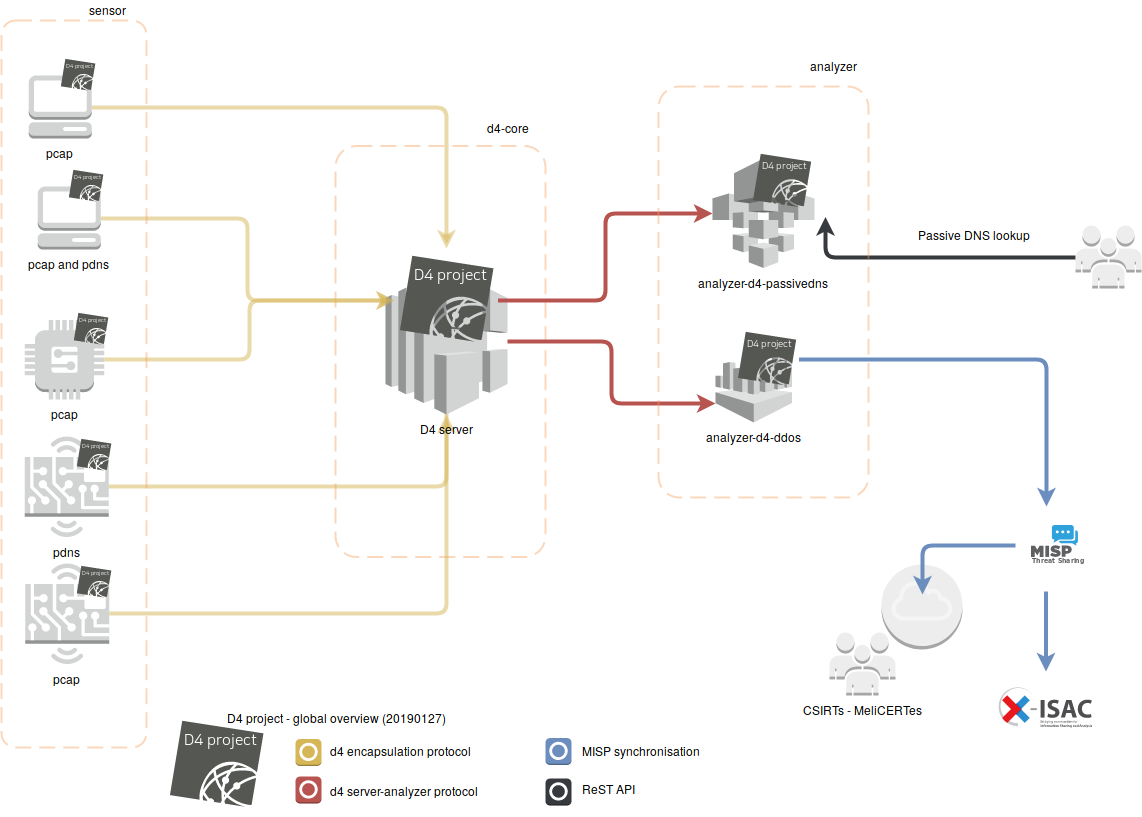
\includegraphics[scale=0.38]{../../diagram/d4-overview.png}
\end{frame}

\begin{frame}
        \frametitle{Roadmap (next 2 months)}
        \begin{itemize}
                \item Passive DNS analyzer (alpha version released)
                \item Passive SSL collector and analyzer
                \item Backscatter DDoS traffic analyzer
                \item {\bf Default server} (blackhole monitoring or Passive DNS collector) at CIRCL for organisations willing to contribute without running their own D4 server
        \end{itemize}
\end{frame}


\begin{frame}
        \frametitle{D4 encapsulation protocol}
        \includegraphics[scale=0.38]{d4-protocol-encapsulation.png}
\end{frame}

\begin{frame}
    \frametitle{D4 Header}
    \begin{tabular}{|l|l|l|}
        \hline
        Name & 	bit size&  	Description\\
        \hline
        version &	uint 8 &	Version of the header \\
        type 	& uint 8   &	Data encapsulated type\\
        uuid 	& uint 128 & 	Sensor UUID\\
        timestamp &  	uint 64 &	Encapsulation time\\
        hmac 	& uint 256 &	Authentication header (HMAC-SHA-256-128)\\
        size 	& uint 32 	& Payload size\\
        \hline
    \end{tabular}
\end{frame}


\begin{frame}
    \frametitle{D4 Header}
    \framesubtitle{Types}
        \begin{tabular}{|l|l|}
            \hline
            Type &	Description\\
            \hline
            0 	& Reserved\\
            1 	& pcap (libpcap 2.4)\\
            2 	& meta header (JSON)\\
            3 	& generic log line\\
            4 	& dnscap output\\
            5 	& pcapng (diagnostic)\\
            6 	& generic NDJSON or JSON Lines\\
            7 	& generic YAF (Yet Another Flowmeter)\\
            8  	& passivedns CSV stream\\
            254 &	type defined by meta header (type 2)\\
            \hline
        \end{tabular}
\end{frame}

\begin{frame}
    \frametitle{D4 meta header}
    \framesubtitle{Meta types}
        D4 header includes an easy way to {\bf extend the protocol} (via type 2) without altering the format. Within a D4 session, the initial D4 packet(s) type 2 defines
        the custom headers and then the following packets with type 254 is the custom data encapsulated.
    \small
    \begin{lstlisting}
{
  "type": "ja3-jl",
  "encoding": "utf-8",
  "tags": [
    "tlp:white"
  ],
  "misp:org": "5b642239-4db4-4580-adf4-4ebd950d210f"
}
\end{lstlisting}

\end{frame}

\begin{frame}
    \frametitle{D4-core server}
   \begin{itemize}
           \item D4 core server\footnote{\url{https://github.com/D4-project/d4-core}} is a complete server to handle clients (sensors) including the decapsulation of the D4 protocol, control of sensor registrations, management of decoding protocols and dispatching to adequate decoders/analysers.
           \item D4 server is written in Python 3.6 and runs on standard GNU/Linux distribution.
   \end{itemize}
\end{frame}

\begin{frame}
\frametitle{D4 server handling}

D4 server reconstructs the encapsulated stream from the D4 sensor and saves it in a Redis stream.

\begin{itemize}
\item Support TLS connection
\item Unpack D4 header
\item Verify client secret key (HMAC)
\item check blocklist
\item Filter by types (Only accept one connection by type-UUID - except: type 254)
\item Discard incorrect data
\item Save data in a Redis Stream (unique for each session)
\end{itemize}
\end{frame}

\begin{frame}
        \frametitle{D4 server - worker handler}
After the stream is processed depending of the type using dedicated worker.
        \begin{itemize}
        \item Worker Manager (one by type)
                \begin{itemize}
                \item Check if a new session is created and valid data are saved in a Redis stream
                \item Launch a new Worker for each session
                \end{itemize}
        \item Worker
                \begin{itemize}
                 \item Get data from a stream
    		     \item Reconstruct data
                 \item Save data on disk (with file rotation)
                 \item Save data in Redis. Create a queue for D4 Analyzer(s)
                \end{itemize}
        \end{itemize}
\end{frame}

\begin{frame}
        \frametitle{D4 server - type 254 worker handler}
        \begin{itemize}
        \item Worker 2
                \begin{itemize}
                \item Get type 2 data from a stream
    		        \item Reconstruct Json
                \item Extract extended type name
                \item Use default type or special extended handler
                \item Save Json on disk
                \item Get type 254 data from a stream
                \item Reconstruct type 254
                \item Save data in Redis. Create a queue for D4 Analyzer(s)
                \end{itemize}
        \end{itemize}
\end{frame}

\begin{frame}
        \frametitle{D4 server - management interface}
The D4 server provides a web interface to manage D4 sensors, sessions and analyzer.
        \begin{itemize}
\item Get Sensors status, errors and statistics
\item Get all connected sensors
\item Manage Sensors (stream size limit, secret key, ...)
\item Manage Accepted types
\item UUID/IP blocklist
\item  Create Analyzer Queues
        \end{itemize}
\end{frame}

\begin{frame}
        \frametitle{D4 server - main interface}
        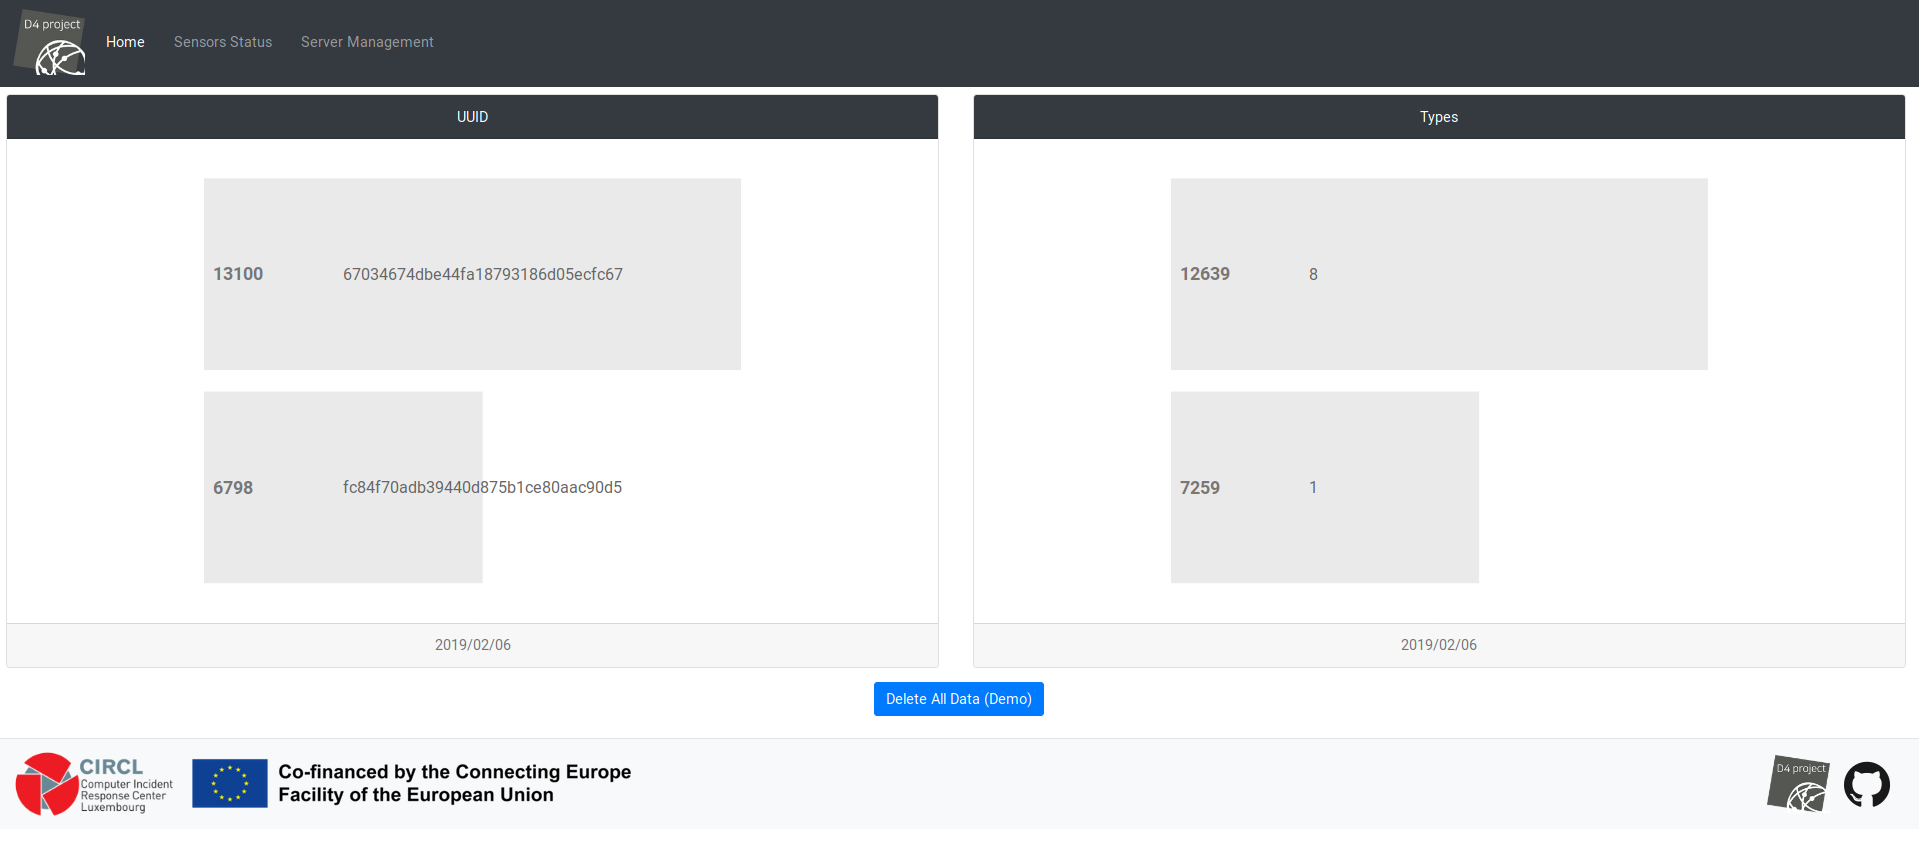
\includegraphics[scale=0.18]{d4-5.png}
\end{frame}

\begin{frame}
        \frametitle{D4 server - server management}
        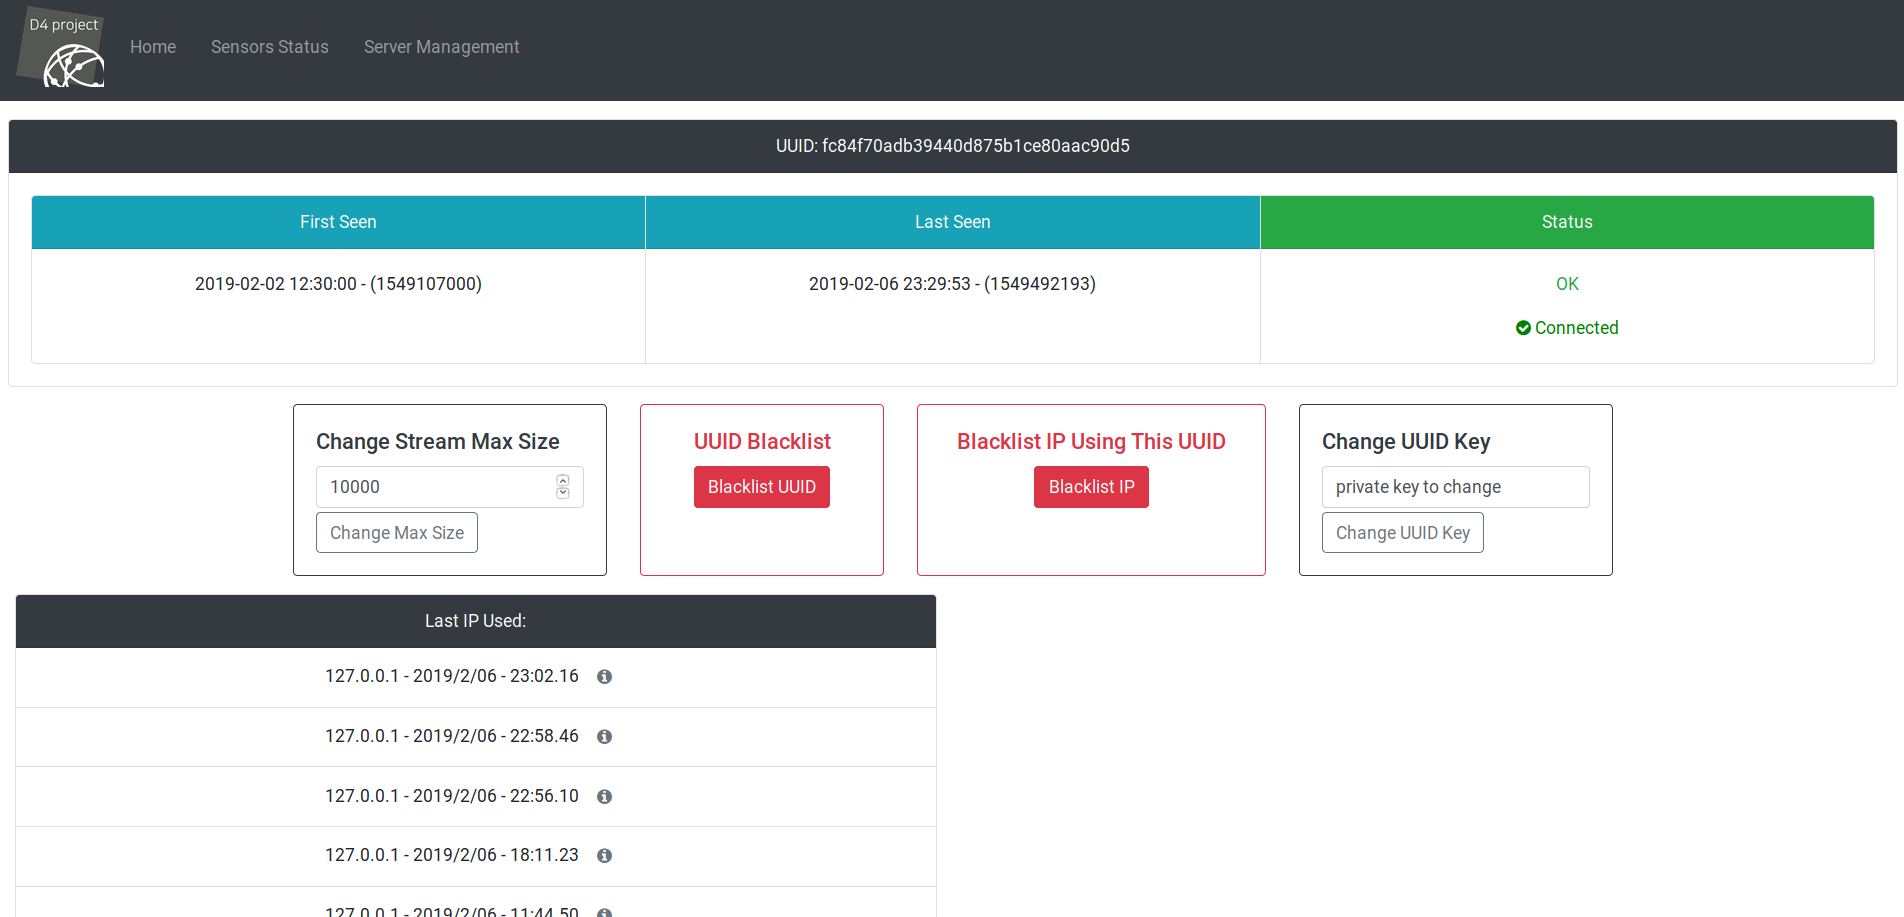
\includegraphics[scale=0.18]{d4-2.png}
\end{frame}

\begin{frame}
        \frametitle{D4 server - server management}
        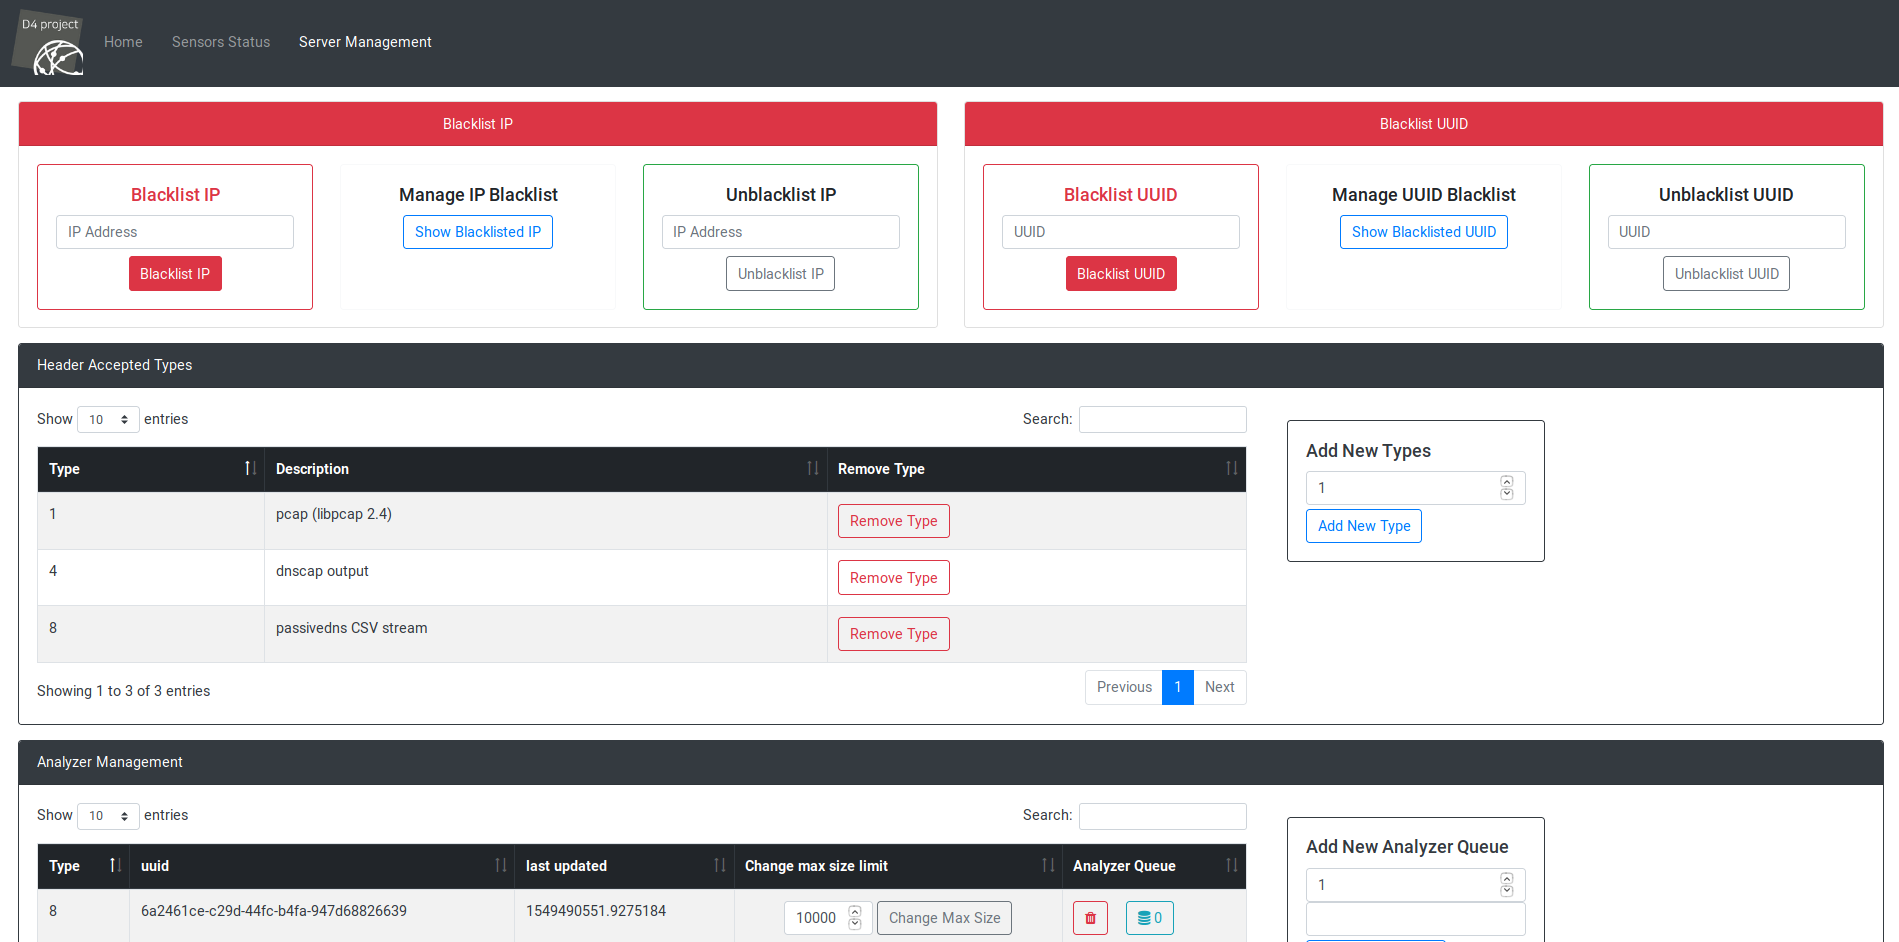
\includegraphics[scale=0.18]{d4-3.png}
\end{frame}

\begin{frame}
        \frametitle{D4 server - sensor overview}
        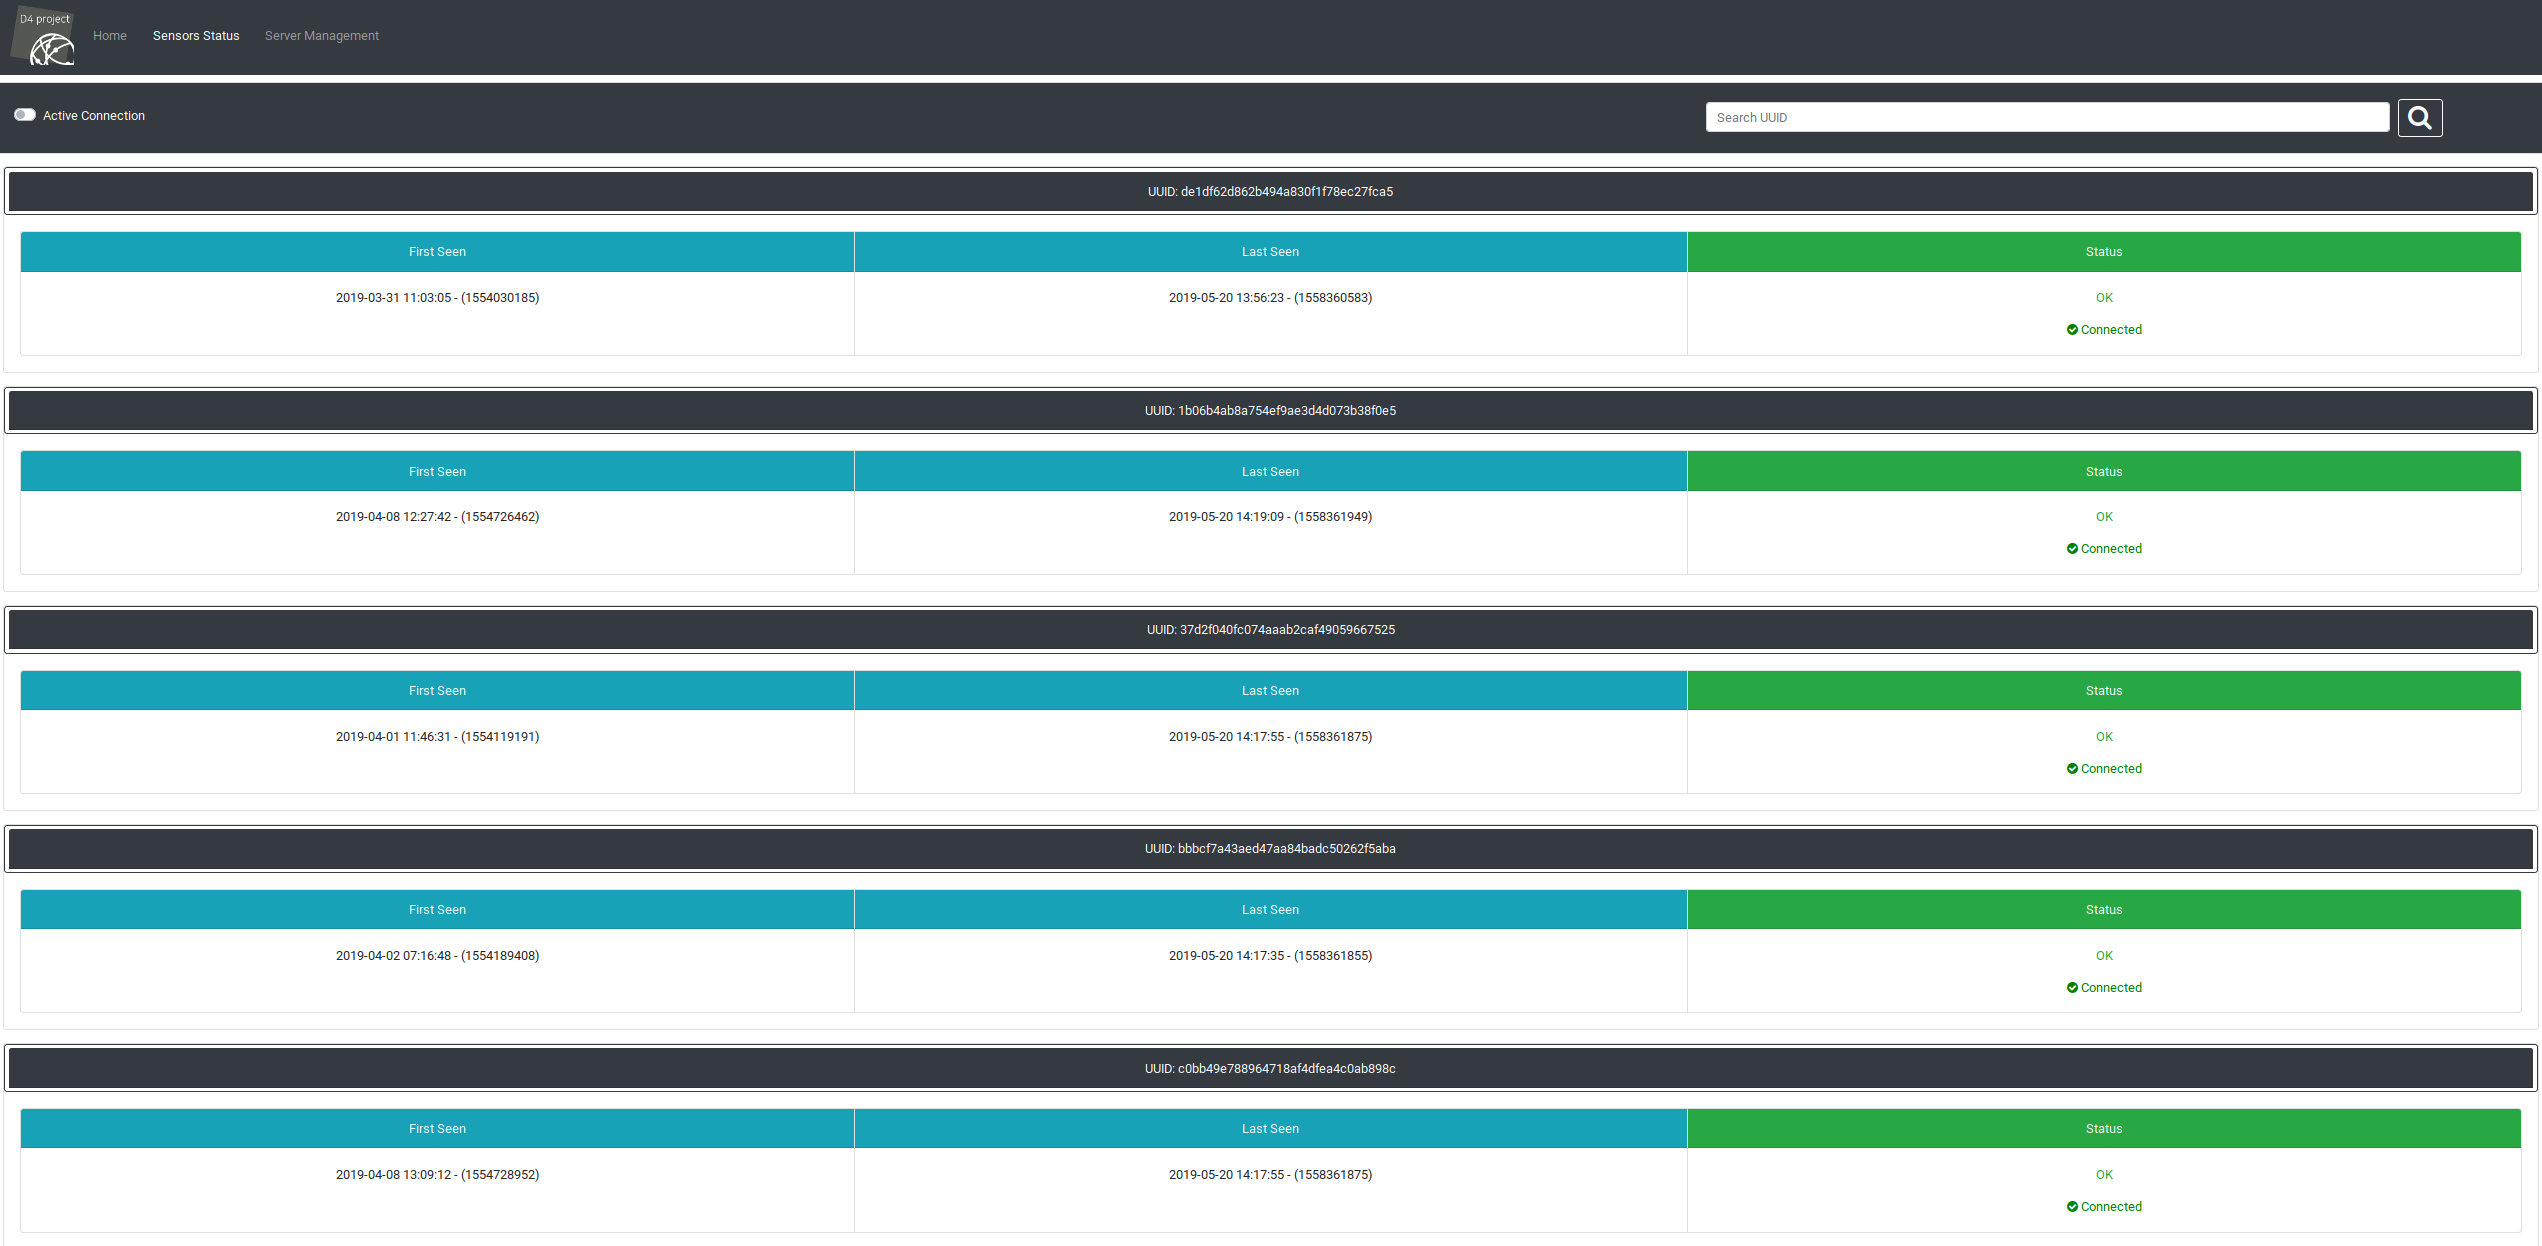
\includegraphics[scale=0.18]{d4-1.png}
\end{frame}


\begin{frame}
        \frametitle{D4 server - sensor management}
        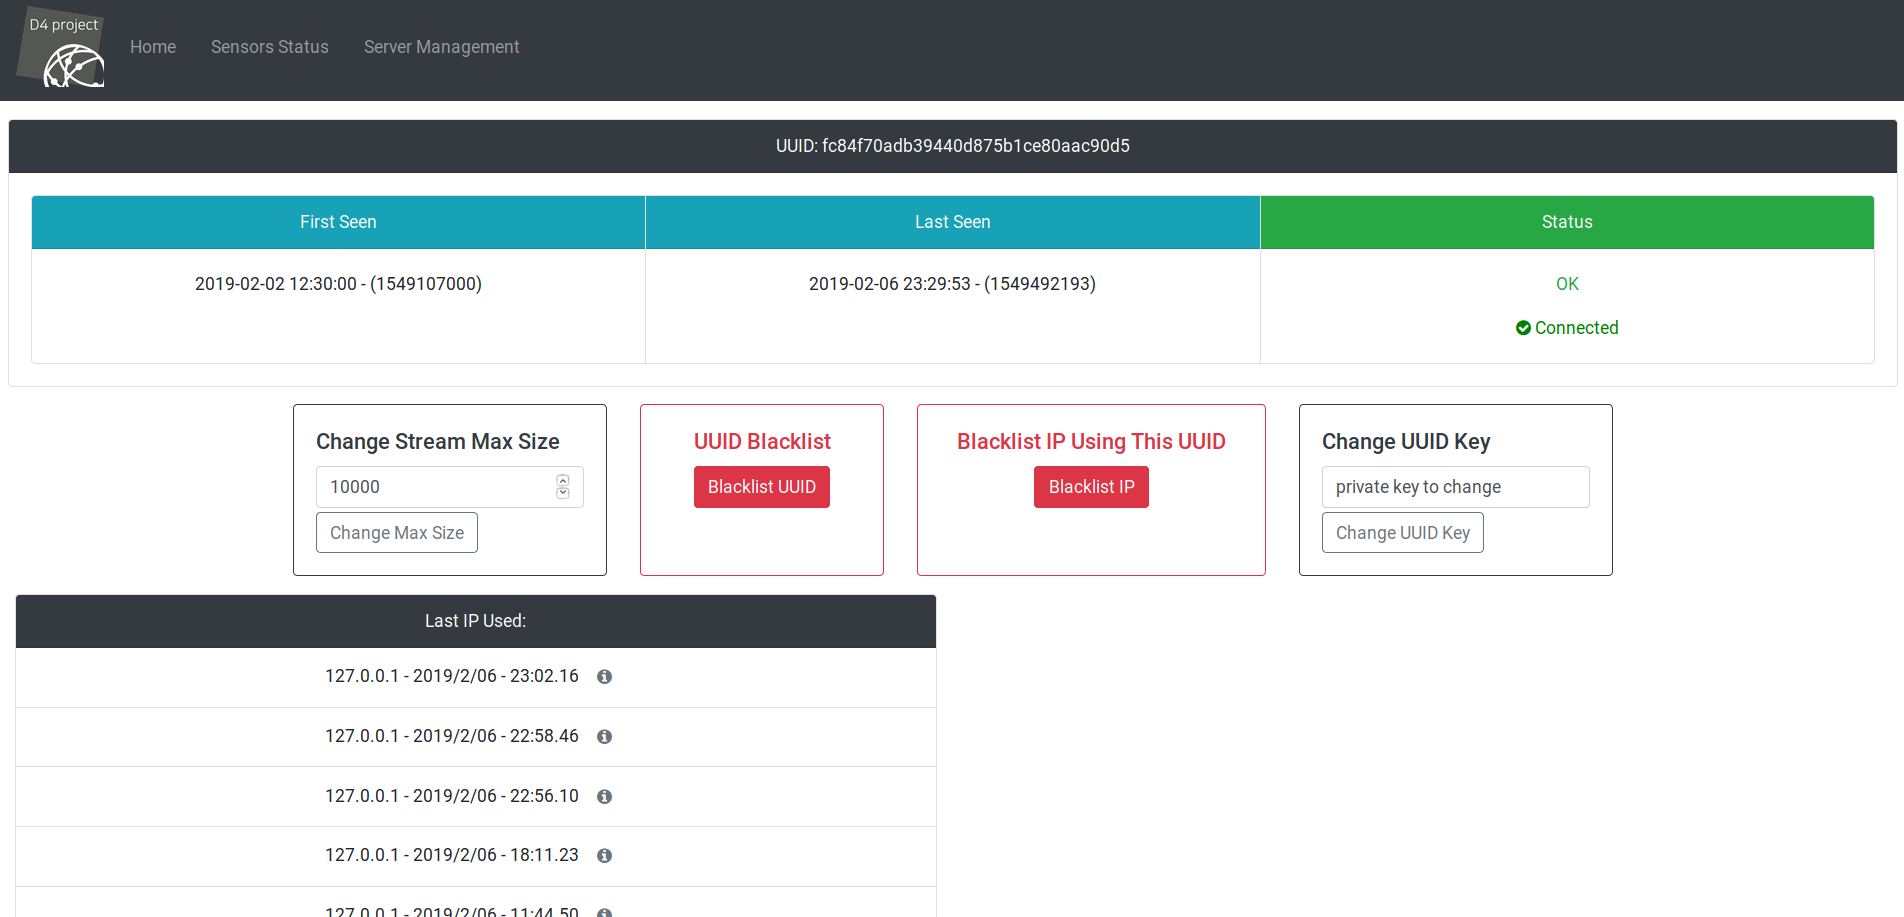
\includegraphics[scale=0.18]{d4-4.png}
\end{frame}



\begin{frame}
        \frametitle{}
        {\center Use-case: migrating a legacy network capture model into a D4 network sensor
}
\end{frame}


\begin{frame}
\frametitle{Remote network capture}
    CIRCL operated honeybot for multiple years using a simple model of remote network capture.
    \begin{definition}[Principle]
        \begin{itemize}
            \item KISS (Keep it simple stupid) - Unix-like
            \item Linux \& OpenBSD operating systems
        \end{itemize}
    \end{definition}

    \begin{block}{Sensor}
    \lstset{%
        language=bash,
        backgroundcolor=\color{gray!25},
        basicstyle=\ttfamily,
        breaklines=true,
        columns=fullflexible
    }
    \begin{lstlisting}
tcpdump -l -s 65535 -n -i vr0 -w - '( not port $PORT and not host $HOST )' | socat - OPENSSL-CONNECT:$COLLECTOR:$PORT,cert=/etc/openssl/client.pem,cafile=/etc/openssl/ca.crt,verify=1
\end{lstlisting}


    \end{block}
\end{frame}

\begin{frame}
    \frametitle{Remote network capture}
    \begin{block}{Limitations}
        \begin{itemize}
            \item Scalability $\to$ one port per client
            \item Identification and registration of the client
            \item Integrity of the data
        \end{itemize}
    \end{block}

    \begin{block}{Encapsulating streams in D4}
        \begin{itemize}
            \item Inspired by the unix command {\tt tee}
            \item Read from standard input
            \item Add the d4 header
            \item Write it on standard output
        \end{itemize}
    \end{block}
\end{frame}


\begin{frame}
    \frametitle{Remote network capture with D4}
    \frametitle{Using D4 native client}
      \lstset{%
        language=bash,
        backgroundcolor=\color{gray!25},
        basicstyle=\ttfamily,
        breaklines=true,
        columns=fullflexible
    }
    \begin{lstlisting}
tcpdump -n -s0 -w - | ./d4 -c ./conf | socat - OPENSSL-CONNECT:$D4-SERVER-IP-ADDRESS:$PORT,verify=1
\end{lstlisting}


\begin{block}{Configuration directory}
    \begin{tabular}{l|l}
        Parameter & Explanation\\
        \hline
        type & see D4 Header slide\\
        source & standard input\\
        key & HMAC key\\
        uuid & Identifier of the sensor\\
        version &  version of the sensor\\
        destination & standard output\\
        snaplen & length of data being read \& written\\
    \end{tabular}
\end{block}
\end{frame}

\begin{frame}
        \frametitle{}
{\center Use-case: D4 analyzer to detect DDoS attacks in backscatter traffic
}
\end{frame}

\begin{frame}
\frametitle{Observing SYN floods attacks in backscatter traffic}
Attack description
    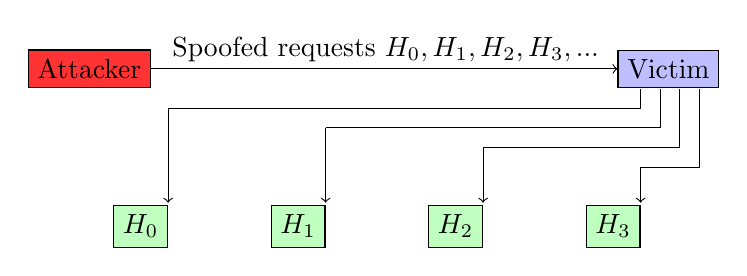
\begin{tikzpicture}{scale=0.4}
    \node[rectangle,draw,fill=red!80] (a) at (0,0) {Attacker};
    \node[anchor=west] at (0.93,0.25) {Spoofed requests $H_{0},H_{1},H_{2},H_{3},...$};
    \node [rectangle,draw,fill=blue!25,anchor=east] at (8,0) (v) {Victim};
    \draw [->](a) --(v);
    \foreach \x in {0,1,2,3} {
        \node [rectangle,draw,fill=green!25,anchor=east] at (\x*2+1,-2) {$H_{\x}$};
        %Horizontal lines
        \draw (\x*2+1, -\x*0.25-0.5)--(7.0+\x*.25,-\x*0.25-0.5);
        %Links to the victim
        \draw (7.0+\x*.25,-\x*0.25-0.5) -- (7.0+\x*.25,-0.25);
        %Links to hosts
        \draw[->] (\x*2+1, -\x*0.25-0.5)--(\x*2+1,-1.70);
    }
    \end{tikzpicture}

\begin{center}
    \begin{tabular}{|l|}
        \hline
        Connections\\
        \hline
        $H_{0}$\\
        \hline
        $H_{1}$\\
        \hline
        $H_{2}$\\
        \hline
        $H_{3}$\\
        \hline
    \end{tabular}
\end{center}
\end{frame}

\begin{frame}
\frametitle{What can be derived from backscatter traffic?}

\begin{itemize}
    \item External point of view on ongoing denial of service attacks
    \item Confirm if there is a DDoS attack
    \item Recover time line of attacked targets
    \item Confirm which services are a target (DNS, webserver, $\dots$)
    \item Infrastructure changes or updates
    \item Assess the state of an infrastructure under denial of service attack
    \begin{itemize}
        \item Detect failure/addition of intermediate network equipments, firewalls, proxy servers etc
        \item Detect DDoS mitigation devices or services
    \end{itemize}
    \item Create probabilistic models of denial of service attacks
\end{itemize}
\end{frame}

\begin{frame}
    \frametitle{Confirm if there is/was a DDoS attack}
    \begin{block}{Problem}
        \begin{itemize}
            \item Distinguish between compromised infrastructure and backscatter
            \item Look at TCP flags $\to$ filter out single SYN flags
            \item Focus on ACK, SYN/ACK, ...
            \item Do not limit to SYN/ACK or ACK $\to$ ECE (ECN Echo)\footnote{\url{https://tools.ietf.org/html/rfc3168}}
        \end{itemize}
    \end{block}
    \lstset{%
    backgroundcolor=\color{gray!25},
    basicstyle=\ttfamily,
    breaklines=true,
    columns=fullflexible
}

\begin{lstlisting}
tshark -n -r  capture-20170916110006.cap.gz -T fields -e frame.time_epoch  -e ip.src -e tcp.flags
1505552542.807286000 x.45.177.71 0x00000010
1505552547.514922000 x.45.177.71 0x00000010
\end{lstlisting}

\end{frame}

\begin{frame}
        \frametitle{Passive Identification of Backscatter (WiP)}
 \lstset{%
        language=bash,
        backgroundcolor=\color{gray!25},
        basicstyle=\ttfamily,
        breaklines=true,
        columns=fullflexible
    }
        \begin{lstlisting}
./pibs -b -r pcap_file.cap
\end{lstlisting}

        Early version is available of PIBS\footnote{\url{https://github.com/D4-project/analyzer-d4-pibs}}
        with a focus on TCP traffic.
\begin{tabular}{l|l}
Options & Explanations\\
\hline
-r & read pcap file\\
-b & display IPs under DDoS on standard output\\
\end{tabular}


\begin{tabular}{l}
	Dependencies\\
	\hline
	libwiretap-dev\\
	libhiredis-dev\\
	libwsutil-dev\\
\end{tabular}
\end{frame}

\begin{frame}
\frametitle{Get in touch if you want to join the project, host a sensor or contribute}
\begin{itemize}
\item Collaboration can include research partnership, sharing of collected streams or improving the software.
\item Contact: info@circl.lu
\item \url{https://github.com/D4-Project} -  \url{https://twitter.com/d4_project}
\end{itemize}
\end{frame}


\end{document}
